\section{Method}

Our approach relies on the well-known observation that the greater the similarity between two projections, the more likely they originated from two 3D particles that adopted close orientations in the ice layer prior to imaging\footnote{Up to some possible intrinsic symmetries of the objects, which are discussed later.}. This principle guides a number of applications in SPA, including that of projection matching~\cite{penczek1994ribosome}.

Taking this line of thought further, we train a function---parametrized as a neural network---to predict the relative orientation between two projections based on their similarity. To make such training possible, we capitalize on our ability to model the cryo-EM imaging procedure to generate a large, representative synthetic dataset using publicly available 3D atomic models.

Using this trained distance function, we can estimate the relative orientations between pairs of projections in any real dataset. Our postulate is that we can then recover, from these estimated relative orientations, the orientations themselves through an appropriate minimization scheme. This two-steps pipeline is illustrated in \figref{schematic-overview}.

\begin{figure}
    \centering
    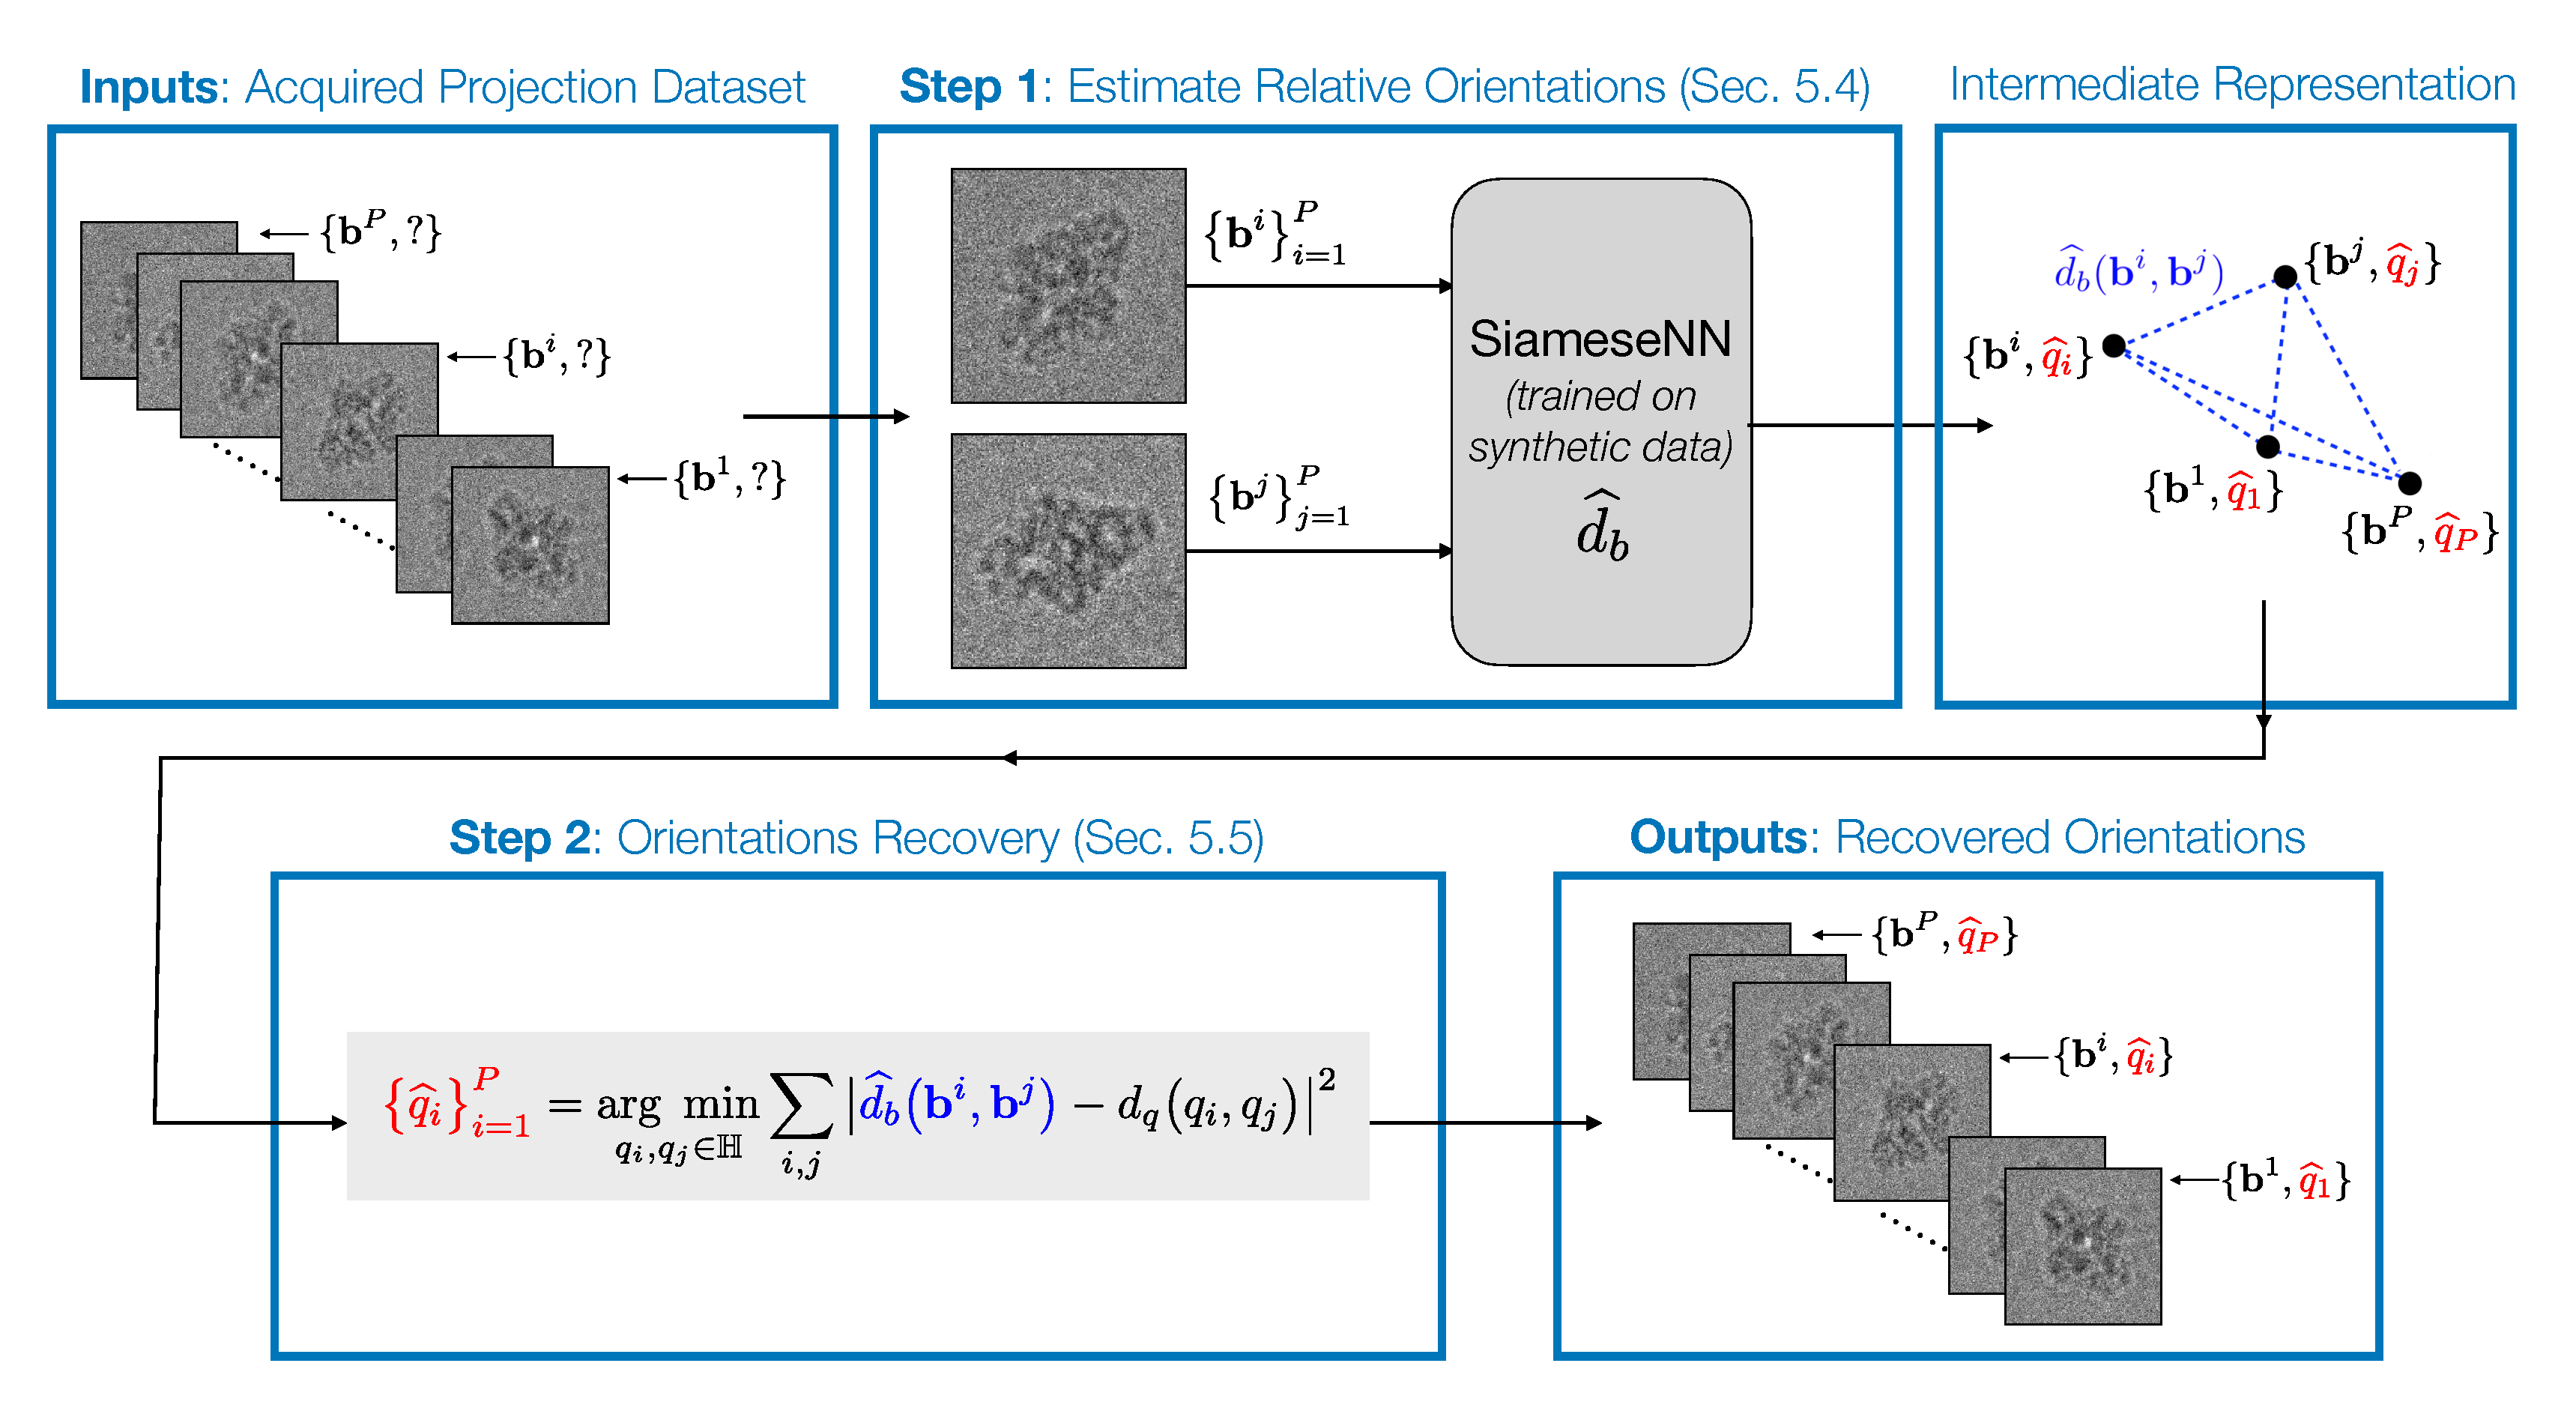
\includegraphics[width=\textwidth]{schematic_overview}
    \caption{Overview of the proposed two-steps method: 1) estimate the relative orientations between projection pairs through a learned distance $\widehat{d}_b$, and 2) recover the orientations from the estimated relative orientations. We denote a $p$th projection by $\mathbf{b}^p$ and its orientation by $q_p$. The geodesic distance between two orientations is denoted by $d_q$.}
    \label{fig:schematic-overview}
\end{figure}

The task of recovering points based on their relative distances has been extensively studied in the literature, mostly within the framework of dimensionality reduction and primarily for the case of \textit{Euclidean} embedding spaces\footnote{An ``embedding space'' corresponds to the (often lower-dimensional) space in which data is embedded, \textit{i.e.}, mapped to in such a way that the relative distances between its points are preserved as much as possible.}~\cite{belkin2003laplacian,kruskal1978multidimensional, maaten2008visualizing, mcinnes2018umap,dokmanic2015euclidean}.
In that respect, the short example given by Dokmanic \textit{et al.} in~\cite{dokmanic2015euclidean} efficiently illustrates the philosophy behind such methods (see the ``An Analogy'' box).
This example, if rather simple, nevertheless underlines well the key ingredients of methods that aim at retrieving points from distances that may not be directly measurable:

\begin{enumerate}
    \item \textit{An appropriate proxy for the ``real'' distance}. In the above example, the proxy for the spatial distance between two cities is the time taken to travel by train between them. In our case, we shall consider the similarity between two projections to be a good proxy for their relative orientation.
    \item \textit{A sufficiently rich collection of proxy distance data}. In this example, these data are provided by the (complete) train timetable. In our approach, we shall estimate the relative orientations between numerous pairs of projections based on the aforementioned proxy distance.
    \item \textit{An efficient recovery scheme}. In~\cite{dokmanic2015euclidean}, the embedding space being Euclidean, the theoretical framework of the Euclidean distance matrices (EDMs) guarantees that one can retrieve the desired points from the collected distances. In our case, as we shall shortly explain, we aim to embed the estimated relative orientations on $\SOThree$, the space of 3D rotations. Unfortunately, the extension of the EDM theory to such manifold is all but straightforward.
\end{enumerate}

There is no simple way to ``handcraft'' a proxy distance that would robustly predict the similarity between two projections. Hence, we resort to \textit{learning} this distance function by parametrizing it as a neural network and capitalizing on 1) the public availability of large datasets of 3D atomic models\footnote{\texttt{https://www.ebi.ac.uk/pdbe/emdb}}, and 2) our ability to model the cryo-EM imaging process. This is the topic of Section~\ref{sec:estimating-relative-orientations}.

Equipped with this learned distance, the idea is then to apply the aforementioned two-steps method (see \figref{schematic-overview}) for any projection dataset. As we just mentioned, we cannot rely on the theoretical framework of EDMs since our embedding space is non-Euclidean. Despite this lack of theoretical guarantees, we are able to appropriately minimize our objective function using a gradient-based algorithm, as we experimentally demonstrate in Section~\ref{sec:orientation-recovery}.

As a preamble, we discuss the need for a representation of orientations in $\SOThree$ that relies on unit quaternions.

\subsection{Unit Quaternions and the Geodesic Distance}
%\subsection{Representation of orientations}
\label{sec:quaternions}

As mentioned, our objective is to recover unknown 3D orientations by embedding their estimated relative distances on the $\SOThree$ space. As we shall explain in the next sections, this embedding requires the efficient computation of the relative distance between two rotations $\mathbf{R}_1, \mathbf{R}_2 \in\SOThree$, which corresponds to the rotation $\mathbf{R}_*\in\SOThree$ such that $\mathbf{R}_1=\mathbf{R}_*\mathbf{R}_2$.

It is standard in SPA to work with Euler angles to describe the orientation of a 3D object in the electron microscope. More precisely, one relies on the parametrization $\bth=(\theta_1,\theta_2,\theta_3)\in\Omega_\bth$, with $\Omega_\bth=[0;2\pi)\times [0;\pi] \times [0;2\pi)$, to encode the 3D rotation that relates the object coordinate system to the projection coordinate system.

Unfortunately, the relative distance between two rotations $\mathbf{R}(\bth_1)$, $\mathbf{R}(\bth_2)$, parametrized by Euler angles cannot be directly computed from $\bth_1$, $\bth_2$. It requires the computation of the rotation matrices, which is computationally inefficient\footnote{Another technical challenge with Euler angles is that they suffer from the so-called gimbal lock problem, which arises when $\theta_2=0$ and restricts the number of rotational degrees of freedom to one even though $\theta_1$ and $\theta_3$ have not yet been fixed~\cite{koks2006explorations}.}. Hence, we resort to a more convenient representation of 3D rotations that relies on unit quaternions.

The algebra of quaternions was introduced in the mid-nineteenth century by Hamilton~\cite{rosenfeld_history_1988}. A quaternion $q\in\mathbb{H}$ takes the form
\begin{equation}
    \label{eq:quaternion-definition}
    q =  a\boldsymbol{1} + b\boldsymbol{i} + c\boldsymbol{j} + d\boldsymbol{k},
\end{equation}
where $(a,b,c,d)\in\mathbb{R}^4$, and $\boldsymbol{1}$, $\boldsymbol{i}$, $\boldsymbol{j}$, and $\boldsymbol{k}$ are the fundamental quaternion units
\begin{equation}
    \label{eq:quaternion-units}
    \boldsymbol{1} = \begin{pmatrix} 1 & 0 \\ 0 & 1 \end{pmatrix}, \quad
    \boldsymbol{i} = \begin{pmatrix} i & 0 \\ 0 & -i \end{pmatrix}, \quad
    \boldsymbol{j} = \begin{pmatrix} 0 & 1 \\ -1 & 0 \end{pmatrix}, \quad
    \boldsymbol{k} = \begin{pmatrix} 0 & i \\ i & 0 \end{pmatrix},
\end{equation}
with $i$ the imaginary unit. Any quaternion $q$ can thus be represented by its set of coefficients $(a,b,c,d)\in\mathbb{R}^4$. The algebra $\mathbb{H}$ is similar to the algebra of complex numbers $\mathbb{C}$, with the exception of the multiplication operation being noncommutative.

In this work, we restrict our interest to unit quaternions $q\in\mathbb{U}$, with  $\mathbb{U}=\big\{q\in\mathbb{H} \; \, | \; \,\lvert q \rvert =1\big\}$, which identify the $\mathbb{S}^3$ hypersphere in  $\mathbb{R}^4$. Unit quaternions concisely and elegantly represent the elements of the $\SOThree$ group. More precisely, a unit quaternion $q\in\mathbb{U}$ parametrizes a rotation $\mathbf{R}\in\SOThree$ through
\begin{equation}
    \mathbf{R}(q) =\begin{pmatrix}
    a^2+b^2-c^2-d^2 & 2bc-ad & 2bd+2ac  \\
    2bc+2ad & a^2-b^2+c^2d^2 & 2cd-2ab \\
    2bd-2ac & 2cd+2ab & a^2-b^2-c^2+d^2
    \end{pmatrix}.
    \label{eq:quaternion-rotation-matrix}
\end{equation}

The geodesic distance $d_q:\mathbb{U}\times\mathbb{U}\rightarrow [0,\pi]$ between two unit quaternions $q_i, q_j\in\mathbb{H}$ is then defined as
\begin{equation}
    \label{eq:geodesic distance}
    d_q(q_i,q_j)=2\arccos\big(|\langle q_i, q_j \rangle|\big),
\end{equation}
with the inner product between quaternions given by
\begin{equation}
    \label{eq:inner-product-quaternions}
    \langle q_i, q_j \rangle = a_ia_j+b_ib_j+c_ic_j+d_id_j.
\end{equation}
The distance~\eqref{eq:geodesic distance} is the shortest distance between $q_i$ and $q_j$ on the surface of $\mathbb{S}^3$.

As $\mathbb{S}^3$ is isomorphic to the universal cover of $\SOThree$, the geodesic distance corresponds to the magnitude of the relative orientation $\mathbf{R}_*$ between $\mathbf{R}(q_i)$ and $\mathbf{R}(q_j)$ in $\SOThree$~\cite{huynh2009metrics}. In other words, the relative distance between two rotations encoded by unit quaternions can be efficiently computed from the unit quaternions themselves through~\eqref{eq:geodesic distance}, which is of key practical importance for this work.

For the sake of conciseness, we shall use the term ``with orientation~$q$'' to refer to 2D/3D objects considered in an imaging geometry parametrized by $q$.

\subsection{Estimating Relative Orientations from Projections}
%\subsection{Relative orientation estimation}
%\subsection{Relative orientation estimation from projections}
\label{sec:estimating-relative-orientations}

Equipped with the geodesic distance $d_q$, our goal is now to find a ``projection distance'' $d_b$ that is a good predictor of $d_q$. Before discussing the different options, we briefly describe the synthetic datasets used in this work.

\subsubsection{Learning $\widehat{d}_b$ with a Siamese Neural Network}

As previously discussed, we make the choice to \textit{learn} a good approximation $\widehat{d}$ on a synthetic training dataset $\big\{ \mathbf{b}^{*p}, q^*_p\big\}_{p=1}^{N_t}$ through
\begin{equation}
    \label{eq:metric-learning-siamese}
    \widehat{d}_b=\argmin{d_b}\sum_{i,j} \big|d_b\big(\mathbf{b}^{*i},\mathbf{b}^{*j}\big) - d_q\big(q^*_i,q^*_j\big) \big|^2,
\end{equation}
with $d_q$ defined in~\eqref{eq:geodesic distance}, and where $N_t$ indicates the number of projection-orientation pairs in the training dataset. More precisely, we parametrize the distance function $d_b$ in~\eqref{eq:metric-learning-siamese} as a Siamese neural network (SiameseNN)~\cite{chopra2005learning}, and resort to learning its weights $w$, as illustrated in \figref{schematic-siamese}.

SiameseNNs, also termed ``twin networks'', are commonly used in the field of deep metric learning to learn similarity functions~\cite{yi2014deep}. They are usually constituted of two sister neural networks that work in tandem and share the exact same architecture and weights.  Their role (once trained) is to extract the projection features that are the most relevant to predict the relative orientation between two projections. The weights $w$ of the two sister networks are progressively learned by 1) comparing the difference of their projection feature vectors to the magnitude of the corresponding relative orientations, and 2) back-propagating this error (via the derivative chain rule) to the weights.

\begin{figure}
    \centering
    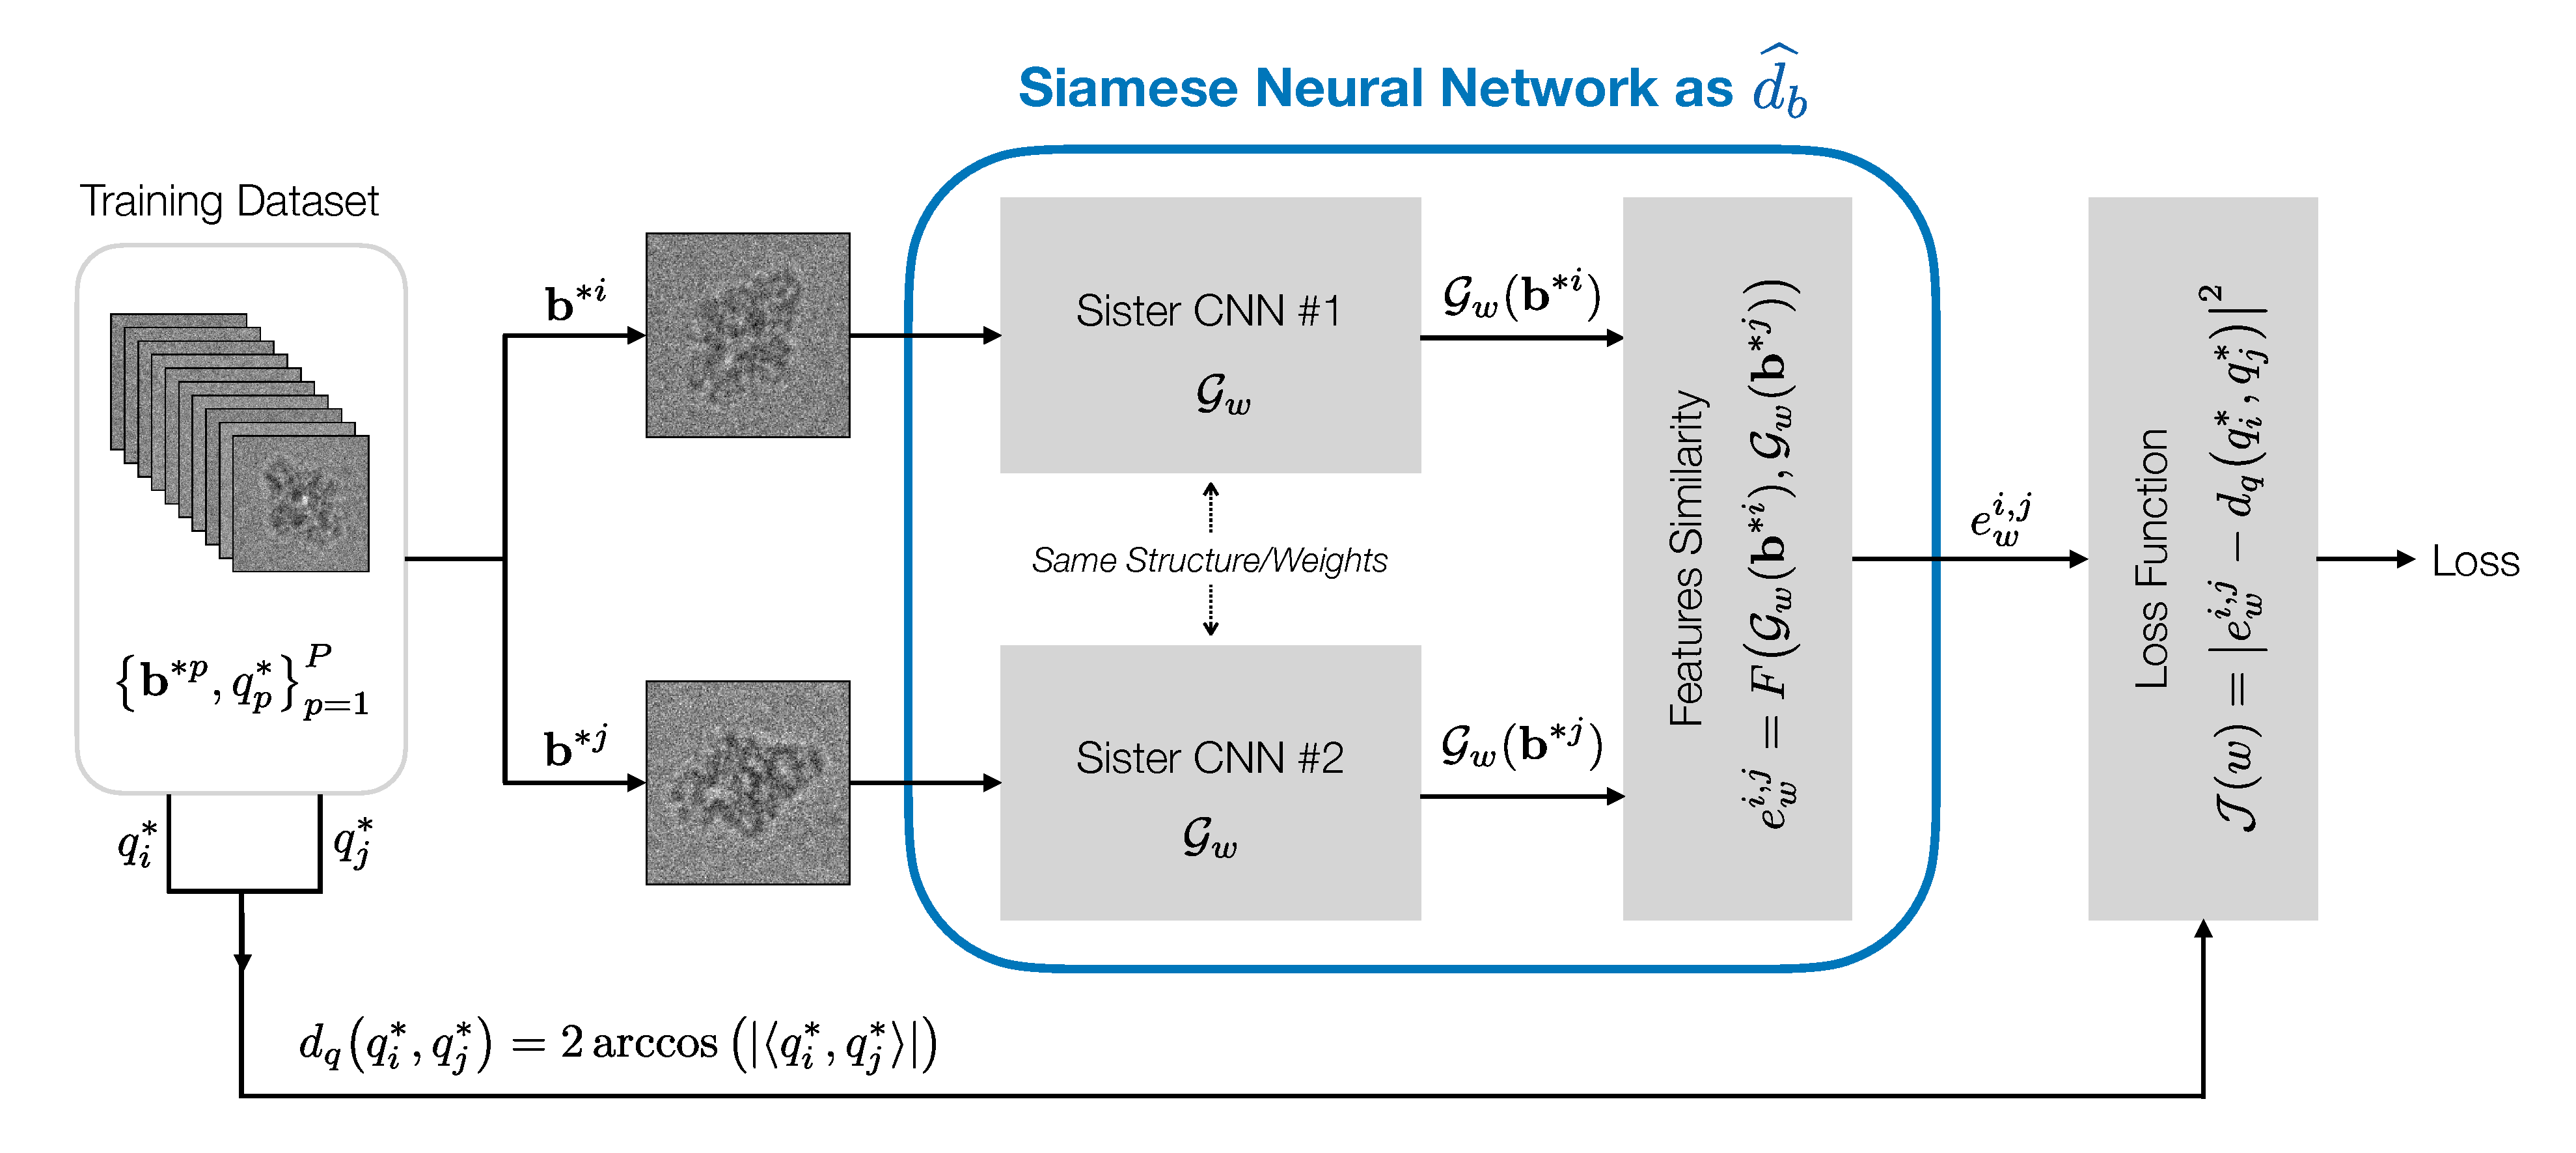
\includegraphics[width=\textwidth]{schematic_siamese}
    \caption{Training a Siamese neural network (SiameseNN) to become a faithful predictor of the relative orientation between two input projections. In other words, we train the SiameseNN to serve as a projection distance $\widehat{d}_b$ that correctly approximates the orientation distance $d_q$. The training is performed with a synthetic dataset that contains thousands of projections with their associated orientation.}
    \label{fig:schematic-siamese}
\end{figure}

\subsection{Orientation Recovery}
%\subsection{Orientation recovery from relative orientations}
\label{sec:orientation-recovery}

Equipped with an appropriately learned $\widehat{d}_b$, the objective is then to recover the unknown unit quaternions $\big\{q_p\big\}_{p=1}^P$ associated to the projections $\big\{\mathbf{b}^p\big\}_{p=1}^P$ in any given dataset.

\subsubsection{Minimization Scheme}

We propose to start this process by computing of a great number of pairwise projection distances $\big\{\widehat{d}_b\big(\mathbf{b}^i,\mathbf{b}^j\big)\big\}_{i,j=1}^{P}$ through $\widehat{d}_b$. Then, our postulate is that we can recover the orientations from theses distances by solving
\begin{equation}
    \label{eq:global-min-problem}
    \big\{\widehat{q}_p\big\}_{p=1}^P=\argmin{q_i\in\mathbb{U}}\sum_{i,j} \big|\widehat{d}_b\big(\mathbf{b}^i,\mathbf{b}^j\big) - d_q\big(q_i,q_j\big) \big|^2,
\end{equation}
as is illustrated in \figref{schematic-overview}.

In practice, one cannot possibly evaluate~\eqref{eq:global-min-problem} for every pair of orientations $\big\{q_i,q_j\big\}_{i,j=1}^P$ given the extremely large size of SPA datasets, with $P$ typically in the order of dozens of thousands. Hence, we need to partially sample the projection dataset. We experimentally demonstrate in Section~\ref{subsec:5-6-3-sanity-check} that this does not affect the performance of our recovery scheme.

As previously discussed, we are not yet aware of any guarantee of convergence for~\eqref{eq:global-min-problem}. Similarly, we do not know of any theoretical characterization of the behaviour of~\eqref{eq:global-min-problem} in ill-posed conditions, such as when pairwise distances are misestimated, for instance. Hence, we rely for now on experimental demonstrations to 1) ensure feasibility, and 2) indicate where efforts need to be invested.

\begin{figure}
    \centering
    \begin{subfigure}[b]{0.48\textwidth}
        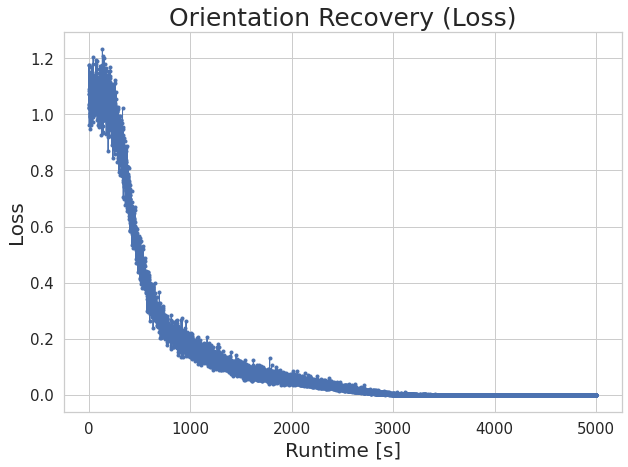
\includegraphics[width=\textwidth]{fig_perfectdistances_loss-symmetric}
        \caption{}
    \end{subfigure} \quad
    \begin{subfigure}[b]{0.48\textwidth}
    \centering
        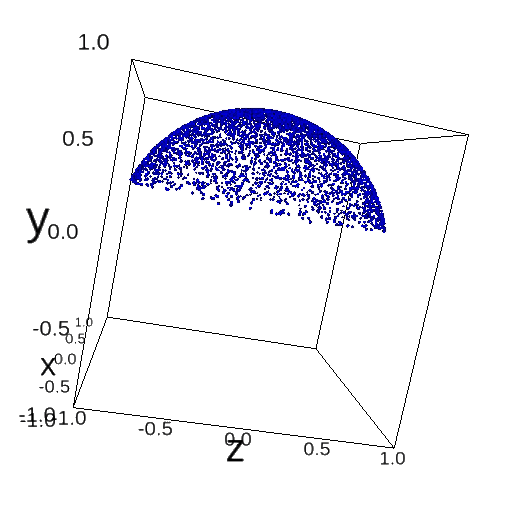
\includegraphics[width=0.8\textwidth]{fig-perfectdistances-coverage-symmetric}
        \caption{}
    \end{subfigure}
    \caption{Results of the orientation recovery scheme when using the perfect orientation distances for the asymmetric protein (5j0n). \textbf{(a)} Evolution of the loss of~\eqref{eq:global-min-problem} during minimization. \textbf{(b)} Coverage of $\SOThree$ after the orientation recovery from the perfect relative distances. }
    \label{fig:minim-loss-perfect-distances}
\end{figure}
